\documentclass[a4paper, 12pt]{article}
\usepackage{a4wide, amsmath, mathtools, amssymb, amsxtra, amsthm, amscd, amsfonts, latexsym}
\usepackage{fullpage}
\usepackage[final]{graphicx}
\usepackage{multirow}
\usepackage{array}
\usepackage{setspace}
\usepackage{appendix}
\usepackage{lscape}
\usepackage{threeparttable}
\usepackage{fancyhdr}
\usepackage{ulem}
\usepackage{algorithm}% http://ctan.org/pkg/algorithm. These two package is used to write algorithm
\usepackage{algpseudocode}% http://ctan.org/pkg/algorithmicx
\usepackage{listings}
\usepackage[english]{babel} % for table %
\usepackage{seqsplit}
\usepackage{subscript}

\begin{document}
\title {Implementation of a polynomial time algorithm to determine relative clique-width of a graph}
\date{April 2012}
\author{Authors: Le Xuan Hoan, Nguyen Huu Phat \\
        \and 
	Supervisors: Professor Bruno COURCELLE and Professor Maylis DELEST}
\maketitle

% ABSTRACT %
\begin{abstract}
Many NP-hard problems are solvable in polynomial time for graphs having a bounded tree width, and correspondingly, having a bounded clique width \cite{vadim-lozin}. Vadim Lozin and Dieter Rautenbach in \cite{vadim-lozin} introduced a polynomial time factor 2 approximation algorithm to determine relative clique width of a graph. And more interestingly this algorithm determines exactly relative clique width with respect to a linear reduced term.

This report is about the implementation of this algorithm for the case of linear reduced terms, as well as about the program we developed to support a visual usage for users.
\end{abstract}

% INTRODUCTION %
\section {Introduction}
Clique width \cite{linear-time} is an important graph parameter in the meaning that many NP-hard problems are solvable in polynomial time for graphs with bounded clique width. However calculating clique width of a graph is NP-complete \cite {np-complete}, it's related to determining the minimum number of labels used in constructing the graph by operations. In \cite {vadim-lozin},  Vadim Lozin and Dieter Rautenbach took a new approach. It deals with another problem, determining relative clique width. In fact clique width of a graph is the minimum of its relative clique widths over all so-called "reduced terms".
\newline\newline Although the authors confirmed that the problem is NP-hard, a polynomial time approximation algorithm was introduced. Moreover the algorithm computes exactly the relative clique width in a special case.
\newline\newline In the next sections, we will give a brief overview about clique width, relative clique width, and the algorithm with a practical example. Then we will explain our implementation for this algorithm

% DEFINATION AND OBJECTIVES %
\section {Definition and Objective}
Hereafter we introduce necessary definitions and notations used in this report, then we will present the algorithm given in \cite{vadim-lozin} for the case of linear reduced term.

%subsection 2.1 clique width%
\subsection{Clique width}
Clique width is an important graph parameter in the sense that many NP-hard problems are solvable for graphs with bounded clique width\newline\newline
Given a simple graph \textit {G(V,E)} (in the context of this articale we only deal with simple, undirected and loop-free graphs), clique width of the graph is defined via labeling vertices of graph and constructing graph through operations. 

\begin{description}
\item [{Definition}] \cite {vadim-lozin} \textit {(labeling a vertex)} \textit {C} is a finite set, a labeled vertex \textit {$v\in V$} is denoted by \textit {i(v)} with $i\in C$, we also call \textit {i(v)} an i-port
\end{description}
Then we have a mapping: 
\[
\gamma:V\rightarrow C
\]
There are three kinds of operations:

\begin{enumerate}
\item Relabeling: denoted by symbol $\rho_{a\rightarrow b}$ : makes all vertices labeled by\textit {a} become labeled by \textit {b} 
\item Edge addition: denoted by symbol $\eta_{a,b}$ : creates edges between vertices labeled by \textit {a} and vertices labeled by \textit {b} 
\item Disjoint union: denoted by symbol $\oplus$ : disjoint union is commutative
\end{enumerate}
The process of constructing graph is denoted as an expression of labeled vertices and these three kinds of operations.  An expression with k labels is called k-expression. In this report we call such an expression a term. 

\begin{description}
\item [{Example}] We use an example from \cite {vadim-lozin}, have a following term
\[
t=\eta_{b,c}(((\rho_{b\to a}(\eta_{b,c}((\eta_{a,b}(a(1)\oplus b(2)))\oplus c(3))))\oplus b(4))\oplus(\eta_{a,c}(\eta_{a,b}(a(5)\oplus b(6)))\oplus c(7)))
\]
\end{description}
This term denotes the following graph:

\begin{figure}[H]
\centering{}
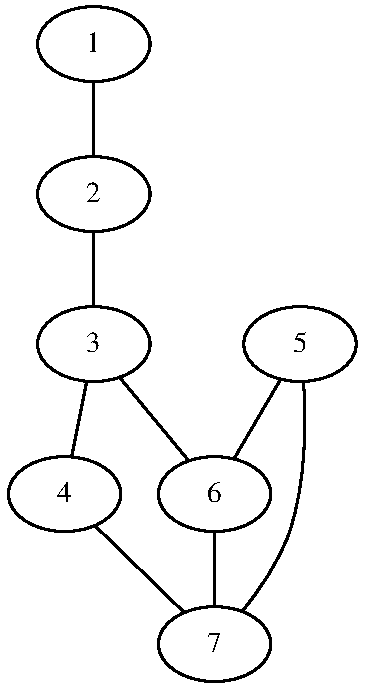
\includegraphics[scale=0.5]{image/graph_by_t}
\caption{Graph by term t}
\end{figure}
Because there may be more than one way to construct a graph, therefore we can have many terms \textit {t }that denote the same graph (two graphs are considered to be the same if they are isomorphic). For such a term \textit {t}, we define \textit {$val(t)=(G,\gamma)$} 

\begin{description}
\item [{Definition}] \cite {vadim-lozin}The \textit {(Clique width)}\textit {cw(G)} of a graph G  is defined as follows: 
\[
cw(G)=min\{\mid C\mid\mid\exists t:val(t)=(G,\gamma)\}
\]
\end{description}
Calculating clique width of a graph is an NP-complete problem.

% section 2.2 Relative clique width%
\subsection{Relative clique width}
Vadim Lozin and Dieter Rautenbach in \cite {vadim-lozin} made a new approach to the problem of determining clique width by introducing the notion of \textit {relative clique width}. 

\begin{description}
\item [{Definition}] \cite {vadim-lozin} \textit {(Reduced term)} a reduced term \textit {r} of a term \textit {t} is a term acquired by replacing in \textit {t} all symbols \textit {i(v)} by \textit {v}, and removing all symbols $\rho_{a\rightarrow b}$ and $\eta_{a,b}$  \item [{Example}] for a term \textit {t} as above, we have the reduced term \textit {r} as follows: 
\[
r=red(t)=(((((((1\oplus2))\oplus 3)))\oplus 4)\oplus(((5\oplus6))\oplus 7))=(((1\oplus2)\oplus3)\oplus 4)\oplus((5\oplus 6)\oplus 7)
\]
\end{description}
This reduced term denotes a rooted binary tree

\begin{description}
\item [{Definition}] \cite {vadim-lozin} \textit {(relative clique width)} relative clique width of a graph G with respect to a reduced term r, \textit {cw(G,r)} is defined as follow: 
\[
cw(G,r)=min\{\mid C\mid\mid\exists t:val(t)=(G,\gamma)\wedge red(t)=r\}
\]
\end{description}
In \cite {vadim-lozin} they introduced a factor 2 algorithm to approximate\textit {cw(G,r)}. An interesting thing is the algorithm can determine exactly in the case reduced terms are linear

\begin{description}
\item [{Definition}] \textit {(linear reduced term)} a reduced term \textit {r} is linear if and only if $\forall$ sub-term $s_{1}\oplus s_{2}$ of r, $\exists i\in\{1,2\}:s_{i}$ has form of \textit {v} 
\item [{Example}] Following is an example of a linear reduced term 
\[
r=(((1\oplus(2\oplus3))\oplus4)\oplus5)\oplus6
\]
\end{description}
This term denotes the following rooted binary tree:\\
\begin{figure}[H]

\begin{centering}
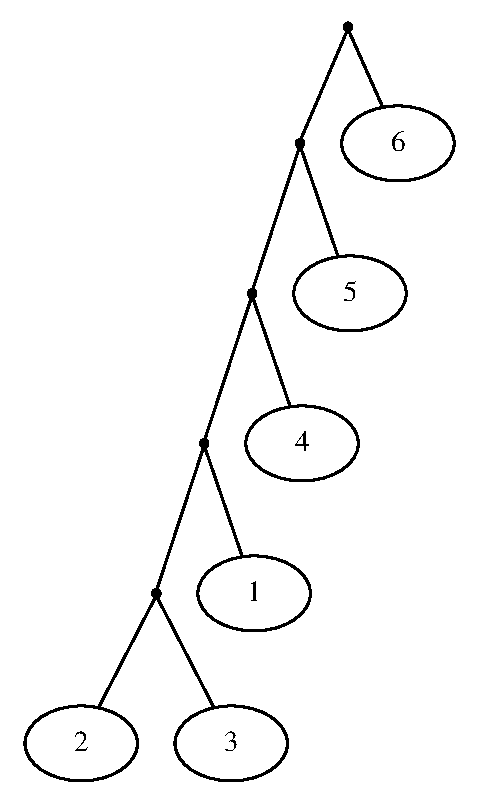
\includegraphics[scale=0.5]{image/tree_by_r}
\caption{Rooted binary tree is used to denote above reduced term r}
\par\end{centering}

\end{figure}

% section 2.3 graph H %
\subsection {Graph H\textsubscript{s}}

In what follows, we introduce a very important notation used in the algorithm, let \textit {$N_{G}(u)$} be the neighborhood of vertex \textit {u} in graph \textit {G} 

\begin{description}
\item [{Definition}] \cite {vadim-lozin} For a sub-term \textit {s} of \textit {r}, let \textit {$V_{s}$} denote the set of vertices in s. We define a graph \textit {$H_{s}=(V_{s}, E(H_{s})$} with $uv\in E(H_{s})\Longleftrightarrow N_{G}(u)\setminus V_{s}\neq N_{G}(v)\setminus V_{s}$
\end{description}
\textit{$H_{s}$} is a complete multi-partite graph (lemma 1 in \cite{vadim-lozin}), let \textit{$H_{s}'$} be the complement graph of \textit{$H_{s}$}, so we have edge relation is an equivalent relation on \textit{$H_{s}'$}

% section 2.4 Algorithm%
\subsection{Algorithm}

This algorithm determines \textit {cw(G, r)} by recursively construction of a term \textit {t} such that \textit {t} satisfies definition of \textit {cw(G,r)}. After that we can approximate \textit {cw(G, r)} (and determine exactly if  \textit {r} is linear). Let \textit {s} is a sub-term of \textit {r}, we construct \textit {t(r)} recursively as follows:

\begin{enumerate}
\item If $s=v\in V$, then $t(s)=i(v),i\in C$ 
\item If $s=s_{1}\oplus s_{2}$, then $t(s)=\beta_{l}(\beta_{l-1}(...(\beta_{1}(\alpha_{k}(\alpha_{k-1}(...(\alpha_{1}(t(s_{1})\oplus t(s_{2})))))))))$, with \textit {$\alpha_{1},...,\alpha_{k}$} have form of $\eta_{i,j}$ and \textit {$\beta_{1},...,\beta_{l}$} have form of $\rho_{i\rightarrow j}$ such that following conditions must be satisfied

\begin{enumerate}
\item \textit {$val(t(s))=(G[Vs],\gamma_{t(s)})$} 
\item \textit {red(t(s)) = s} 
\item $\forall u,v\in V_{s},\gamma_{t(s)}(u)=\gamma_{t(s)}(v)\Leftrightarrow uv\notin E_{s}$,
it means \textit {$\gamma_{t(s)}$}assigns the same label to two vertices iff they stay in the same partite set of \textit {$H_{s}$} 
\item \textit {$\gamma_{t(s_{1})}\cap\gamma_{t(s_{2})}=\emptyset$} \end{enumerate}
\end{enumerate}
Algorithm 1 is the pseudo-code of a recursive function constructing a term for a linear reduced term {$s=rTerm\oplus vertex$}. This function uses some notations of Java programming language

\begin{algorithm}
\caption{Term constructing algorithm}
\begin{algorithmic}[1]
\Function{constructTerm}{$rTerm, vertex$, graph}
	\If {$rTerm\ \textbf{is}\ ProperTerm$}
		\State {$leftTerm \gets constructTerm(rTerm.left, rTerm.right)$}
	\Else
		\State  {$leftTerm \gets constructPort(rTerm)$}
	\EndIf
	\State {$port \gets constructPort(vertex)$}
	\State {$usedLabels \gets leftTerm.usedLabels \cup port.usedLabels$}
	\Comment{usedLabels is the set of labels is used in this term}
	\State {$V_{s} \gets leftTerm.vertexSet \cup port.vertexSet$}
	\State {$constructHs(V_{s})$, graph}
	\State partites {$\gets$} constructHsPartites(leftTerm.partites{$\cup$}port.partites)
	\State {$gammaImage \gets \emptyset$}
	\Comment{gammaImage will be $\gamma_t(s)$}
	\State operatorList {$\gets$} constructOperatorList(leftTerm, port,
                partites, graph, gammaImage)\linebreak
	\Comment{constructOperatorList returns list of operators of a term, and computes the image of mapping $\gamma_t(s)$ as well}
	\State \Return \textbf{new}\ ProperTerm(snTerm, port, termVs, usedlabel,
                gammaImage, partites, operatorList);
\EndFunction
\end{algorithmic}

\end{algorithm}
With condition (c), we need to determine partite sets of \textit {$H_{s}$}. Fortunately, we get an algorithm to do that from Lemma 2 in \cite {vadim-lozin} : 

\begin{quotation}
If $s=s_{1}\oplus s_{2}$ is a sub-term of r, then every partite sets of \textit {$H_{s}$}is a union of partite sets of $H_{s_{1}}$ and $H_{s_{2}}$ 
\end{quotation}

\begin{quotation}
Call $U_{s_{1}}$and $U_{s_{2}}$is sets of partite set of $H_{s_{1}}$ and $H_{s_{2}}$, we have Algorithm 2 as follows:
\end{quotation}

\begin{algorithm}[H]
\caption{Partite sets determining algorithm}
\begin{algorithmic}[1]
	\State $U\gets U_{s_{1}} \cup U_{s_{2}}$ 
	\While{$U\neq\emptyset$}
		\State $partiteSets\leftarrow\emptyset$ \Comment{partiteSets will contain partite sets of $H_{s}$ }
		\ForAll{$u\in U$}
			\State $vertexU\gets u.get(0)$
			\ForAll{$vertex\in vertexSet$}
				\State $contained\gets true$
				\If{$(vertex,vertexU)\in E(H_{s})$}
					\State $contained\gets false$
					\State break
				\EndIf
			\EndFor
			\If{$contained$}
				\State $partiteSets.add(u)$
				\State $U.remove(u)$
			\EndIf
		\EndFor
	\EndWhile 
\end{algorithmic}
\end{algorithm}

% section 2.5 A practical example%
\subsection{A practical example}

To make an example, we will run manually the relative clique determining algorithm with following input:
\begin{itemize}
\item A Graph with 6 vertices\\
 
\begin{figure}[H]
\centering{}
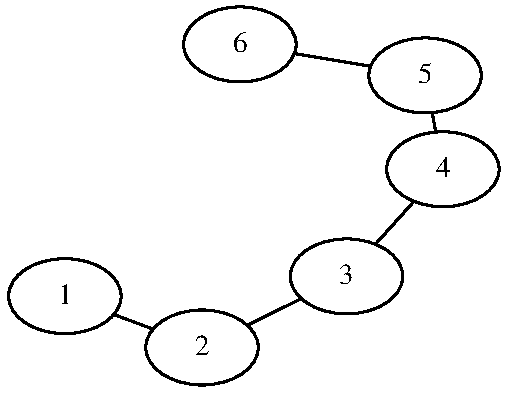
\includegraphics[scale=0.5]{image/graph_example}
\end{figure}

\item Linear reduced term $r=(((1\oplus(2\oplus3))\oplus4)\oplus5)\oplus6$
\item Set of label \textit {\{'a', ..., 'z'\}}
\end{itemize}

It's easy to see that actually the algorithm does the recursion on the structure of \textit {s} (a tree-like structure). However to keep the illustration for this algorithm clear and simple, instead of going
top-down from the root of the tree, we will describe the illustration directly, bottom up from the deepest leaves (see an example of a rooted binary tree above).\pagebreak
\begin{enumerate}
\item \textit {s = 2}

\begin{itemize}
\item We have: \textit {a(2)}
\item {$V_s$}= \{2\}
\item {$H_s$}= 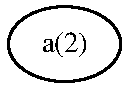
\includegraphics[scale=0.5]{image/example1}
\item \textit {t(s) = a(2)}
\item U({$H_s$}, 1) = \{a(2)\}
\item $\gamma_{t(s)}(V_{s})=\{a\}$ 
\end{itemize}

\item \textit {s = 3}
\begin{itemize}
\item ...
\end{itemize}

\item $s=2\oplus3$
\begin{itemize}
\item We have: $a(2)\oplus b(3)$
\item Apply (a) $\Longrightarrow\eta_{a,b}(a(2)\oplus b(3))$
\item {$V_s$}= \{2, 3\} 
\item {$H_s$}= 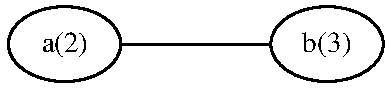
\includegraphics[scale=0.5]{image/example3}
\item U({$H_s$}, 1) = \{a(2)\}, U({$H_s$}, 2) =
\{b(3)\} 
\item $t(s)=\eta_{a,b}(a(2)\oplus b(3))$ 
\item $\gamma_{t(s)}(V_{s})=\{a,b\}$ 
\end{itemize}

\item $s=1\oplus(2\oplus3)$
\begin{itemize}
\item ...
\end{itemize}

\item $s=(1\oplus(2\oplus3))\oplus4$
\begin{itemize}
\item ...
\end{itemize}

\item $s=((1\oplus(2\oplus3))\oplus4)\oplus5$
\begin{itemize}
\item ...
\end{itemize}

\item $s=(((1\oplus(2\oplus3))\oplus4)\oplus5)\oplus6$
\begin{itemize}
\item We have: $\rho_{c\rightarrow a}(\eta_{b,c}(\rho_{b\rightarrow a}(\eta_{c,b}(\rho_{c\rightarrow a}(\eta_{c,a}(c(1)\oplus\eta_{a,b}(a(2)\oplus b(3))))\oplus c(4)))\oplus b(5)))\oplus c(6)$
\item Apply (a) $\Longrightarrow\eta_{c,b}(\rho_{c\rightarrow a}(\eta_{b,c}(\rho_{b\rightarrow a}(\eta_{c,b}(\rho_{c\rightarrow a}(\eta_{c,a}(c(1)\oplus\eta_{a,b}(a(2)\oplus b(3))))\oplus c(4)))\oplus b(5)))\oplus c(6))$
\item {$V_s$}= \{1, 2, 3, 4, 5, 6\} 
\item {$H_s$} = 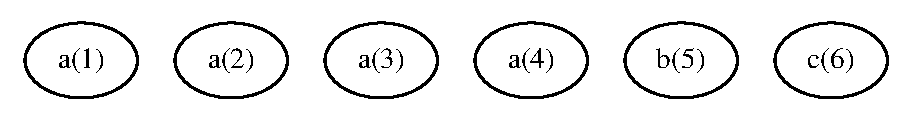
\includegraphics[scale=0.5]{image/example7}
\item U({$H_s$}, 1) = \{a(1), a(2), a(3), c(4), b(5), c(6)\} 
\item Apply (c) $\Longrightarrow t(s)=\rho_{c\rightarrow a}(\rho_{b\rightarrow a}(\eta_{c,b}(\rho_{c\rightarrow a}(\eta_{b,c}(\rho_{b\rightarrow a}(\eta_{c,b}(\rho_{c\rightarrow a}(\eta_{c,a}(c(1)\oplus\eta_{a,b}(a(2)\oplus b(3))))\oplus c(4)))\oplus b(5)))\oplus c(6))))$ 
\item $\gamma_{t(s)}(V_{s})=\{a\}$ 
\end{itemize}
\end{enumerate}
For full details of running steps, see Appendix A.\newline
We have other test cases for the same graph as above, see Appendix B.\newline
We also have test cases with another graph, see Appendix C.

% 3. IMPLEMENTATION THE ALGORITHMS %
\section {Implementation of the algorithm}
This section is an introduction about the work we have done, develop a program to realize this algorithm. First of all we will summarize the requirements from our advisor, then introduce briefly the program.

%section 3.1 Requirement specification}%
\subsection{Requirement specification}

The program takes following inputs: 
\begin{itemize}
\item The number of vertices of a graph
\item The list of edges of the graph, for example: \textit {((1, 2) , (2, 3) , (3, 4) , (4, 5) , (5, 6))}
\item A linear reduced term r. We denote graph operators in ASCII sequence as follows:
\begin{itemize}
\item \textit {oplus(..., ...)} for $...\oplus...$
\item \textit {rel\_a\_b} for $\rho_{a\rightarrow b}$
\item \textit {add\_a\_b} for $\eta_{a,b}$
\end{itemize}

For example\textit { }oplus(oplus(oplus(oplus(1,oplus (2, 3)), 4) , 5),6). To leverage the input readability, two types of parenthesis, \textit {()} and \textit {{[}{]}} are supported, it means someone can input oplus{[}oplus{[}oplus(oplus(1, oplus (2, 3)),4), 5{]}, 6{]}
\end{itemize}
The program will output a term \textit t such that \textit {$val(t)=(G,\gamma)$} and \textit {red(t) = r} and the number of labels used in t is minimum. For example, with the reduced term r as above, the program will output: \textit{\seqsplit{rel\_c\_a[rel\_b\_a[add\_c\_b[oplus(rel\_c\_a[add\_b\_c[oplus(rel\_b\_a[add\_c\_a[oplus(rel\_c\_b[add\_c\_b[oplus(add\_b\_a[oplus(a(3),b(2))],c(1))]],c(4))]],b(5))]],c(6))]]]}}


%section 3.2 Program specification}%
\subsection{Program specification}

Our program is provided in two user interfaces: a console UI (User interface) and a graphical UI (GUI)
\begin{enumerate}
\item Console UI:
\begin{itemize}
\item The usage is as follows:\\
{$rcw.(bat|sh)\ input.txt\ [output.txt]$}

\item In the case output file is missing, term t will be printed out to
console 
\end{itemize}

\item Graphical UI (User Interface):
\begin{itemize}
\item We provide a GUI (Graphic User Interface) version of the program, to start it, just run:\\
{$rcwui.(bin|sh)$}
\item Following is a screen-shot of this GUI\\

\begin{figure}[H]
\begin{centering}
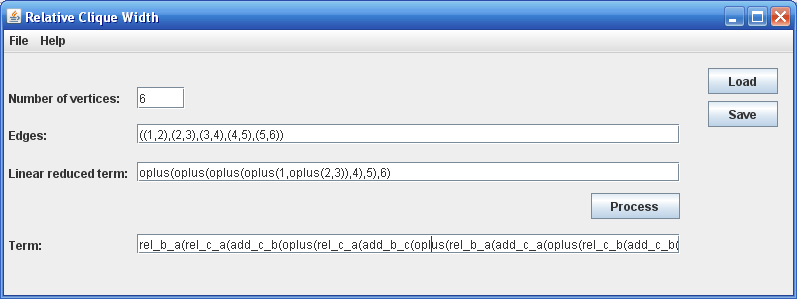
\includegraphics [width=15cm]{image/MainUi.PNG}
\caption{The main form of program}
\par\end{centering}

\end{figure}

\end{itemize}
\end{enumerate}

% 4. METHODS AND USED TOOLS %
\section {Methods and used tools}
Now is the time for us to look deeper into the details of implementation. Throughout this section, we will provide informations about the programming language, the processing of input data, and the data structure (or according to object oriented programming, the class diagram) we used

%section 4.1 Programming language%
\subsection{Programming language}
Our choice of programming language is Java. Java is a platform-independent language, so our program can run seamlessly on any operation system that supports Java (Windows, Linux, Mac OS ...).\newline\newline
Beside that Java has a very big user-community, so we can find support from community for common problems we can cope with during implementation process. For example, to process data input, which we are about to discuss right after, we utilize a lexer/parser generator from public domain

% section 4.2 Processing of data input%
\subsection{Processing of data input}

As mentioned above, we have three types of input data 
\begin{enumerate}
\item The number of vertices of a graph 
\item The list of edges of the graph, for example: \textit {((1,2),(2,3),(3,4),(4,5),(5,6))}
\item A linear reduced term \textit {r}, for example:\textit {oplus(oplus(oplus(oplus(1,oplus(2,3)),4),5),6)}. To leverage the input readability, two types of parenthesis, () and {[}{]} are supported, e.g. someone can input \textit {oplus{[}oplus{[}oplus(oplus(1,oplus(2,3)),4),5{]},6{]}}
\end{enumerate}
Processing of (1) is trivial, (2) is less easy, and (3) is a bit difficult. Fortunately, we could overcome this problem quite quickly with so-called parser generator, and more fortunately, there are such
generators for Java. The one we chose is JavaCC \footnote {http://java.net/projects/javacc} - stands for Java Compiler Compiler, a very popular parser generator for Java. JavaCC takes a grammar specification written in Extended Backus Naur Form (EBNF), and then generates Java source code of the corresponding parser. JavaCC also comes with a specific tools JJTree \footnote {http://www.j-paine.org/dobbs/jjtree.html}, which helps to build an Abstract Syntax Tree (AST) from data input to parser. So all the works we must do are just writing the context free grammar for (2) and (3) 

\begin{itemize}
\item Edge list
\begin{lstlisting}
COMMA = ",";
LP = "(";
RP = ")";
NUMBER = ['0'-'9']+;
VERTEX = NUMBER;
EDGE = LP VERTEX COMMA VERTEX RP;
EDGELIST = LP EDGE COMMA EDGE* RP;
\end{lstlisting}

\item Linear reduced term
\begin{lstlisting}
OPLUS = "oplus";
LP = "(";
RP = ")";
LSB = "[";
RSB = "]";
COMMA = ",";
NUMBER = (["0"-"9"])+;
VERTEX = NUMBER;
REDUCEDTERM = VERTEX |
      <OPLUS> <LP> VERTEX <COMMA> REDUCEDTERM <RP> |
      <OPLUS> <LP> REDUCEDTERM <COMMA> VERTEX <RP> |
      <OPLUS> <LSB> VERTEX <COMMA> REDUCEDTERM <RSB> |
      <OPLUS> <LSB> REDUCEDTERM <COMMA> VERTEX <RSB>;
\end{lstlisting}
 
\end{itemize}

% section 4.3 {Data structure}%
\subsection{Data structure}

Java is an OOP \footnote {Object-Oriented Programming} language, so to install the algorithm in Java, we need
to realize the incident notations to the algorithm (such as term,
graph) as Java classes. Following are class diagrams related to these
notations:

% section 4.3.1 {Class diagram for term-related notations}%
\subsubsection{Class diagram for term-related notations}

\begin{figure}[H]

\begin{centering}
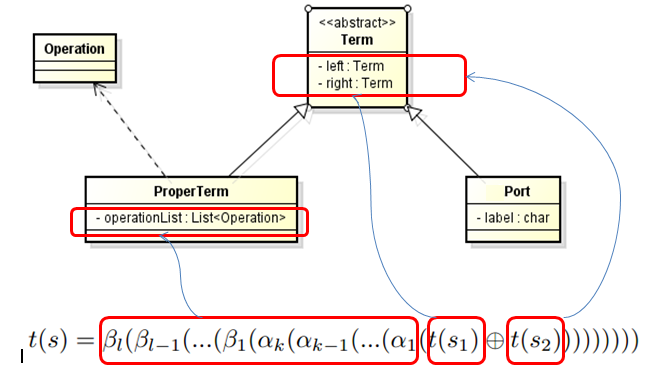
\includegraphics[scale=0.6]{image/classdiagram1}
\caption{Class diagram for \textbf {term-related notations}}
\par\end{centering}

\end{figure}
Some annotations:
\begin{itemize}
\item Port is class for terms \textit {t(s)} with \textit {s = v}
\item ProperTerm is class for terms \textit {t(s)} with $s=s_{1}\oplus s_{2}$
\end{itemize}

% section 4.3.2 {Class diagram for graph-related notations}%
\subsubsection{Class diagram for graph-related notations}

\begin{figure}[H]
\centering{}
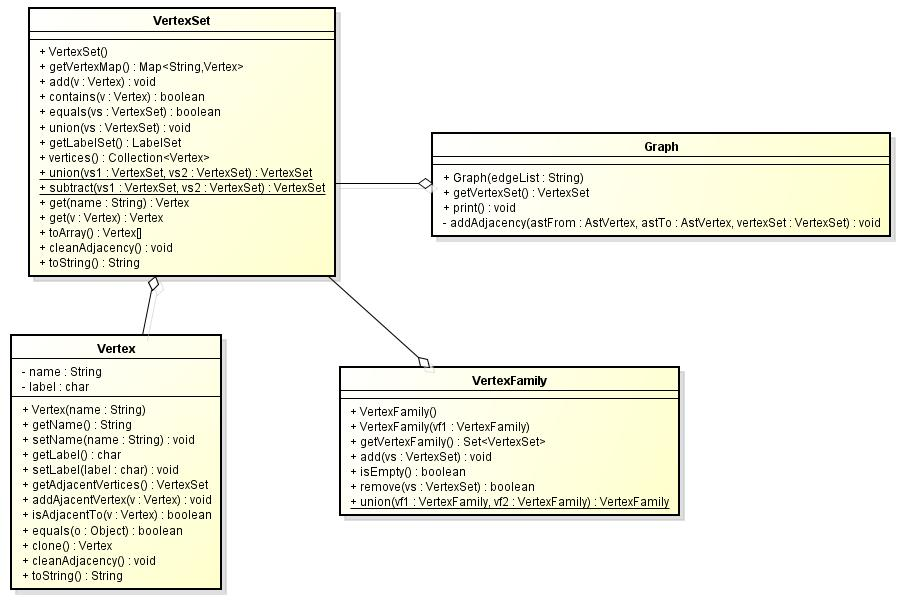
\includegraphics[scale=0.6]{image/classdiagram2.png}
\caption{Class diagram for\textbf {graph-related notations}}
\end{figure}

Some annotations:
\begin{itemize}
\item \textit {Vertex} is class to abstract a vertex, each vertex has a list of adjacent vertices
\item \textit {VertexSet} is a class to abstract a set of vertices, \textit {VertexSet} supports some set operations such as subtract, union
\item \textit {VertexFamily} is a set of sets of vertices. We use \textit {VertexFamily} to denote notations such as \textit {set of partite sets}
\end{itemize}

% section 4.6 {Source code version control system}%
\subsection{Source code version control system}

We also setup a central source code repository for development process. The version control system we use is Git.\newline
Our source code is hosted on github at https://github.com/pufm2/rcw

% RESULTS %
\section {Result}
We tested this program with some data tests as follows, program works fine all cases. You can find these tests in Appendix B and C


% CONCLUSION %
\section {Conclusion}
The program basically meets the requirements, it is able to determines exactly relative clique width of a graph with respect to a linear reduced term. However, as mentioned above, there are still many things waiting to improve, especially about usability of the program.\newline\newline
The program basically satisfies the requirements. However the user interface is not really user-friendly and the usability should be improved. For example, to increase usability, there are many things the program could handle:
\begin{itemize}
\item Support drawing graph 
\item Mapping from a sub-term of \textit {r} to the corresponding sub-graph 
\item Output the result step-by-step like the example we did above, so user
can easily verify the result 
\end{itemize}
Clique width as well as other parameters of graph is an interesting subject. Researching in this field is quite valuable. During this project, we have been aware that there are more effective algorithms to approximate clique width. So we believe one of further works we could try is to investigate those algorithms.

% ACKNOWLEDGEMENTS %
\section {Acknowledgements}
We would like to say a deep thank to Professor Bruno COURCELLE – who has raised a very interesting project for us, graph decomposition, clique-width and their related problems were not familiar for us before and were not easy for us during the project. But with a continuous and enthusiastic support from Professor Courcell, we overcame many troubles and found our pleasure for the subject.\newline\newline
Needless to say there are also many thanks from us  to Professor Maylis DELEST- who taught us how to plan a researching project and write a professional report, Professor Olivier BAUDON - who spent a lot of time to make us clear about this subject when he came to Viet Nam.\newline\newline
We also thank our classmates for their encouragements during our project.

% BIBLIOGRAPHY %
\begin{thebibliography}{99}
\bibliographystyle{abbrv}

\bibitem{vadim-lozin}  Vadim Lozin, Dieter Rautenbach, "The relative clique-width of a graph", \textit{Journal of Combinatorial Theory, Series B}, pp. 846-858, 2007.

\bibitem{upper-bounds} Bruno Courcelle, Stephan Olariu, "Upper bounds to the clique width of graphs", \textit{Discrete Applied Mathematics}, pp. 77-114, 2000.

\bibitem{automata} Bruno Courcelle, "Automata for monadic second-order model-checking", Bordeaux, France, 2011.

\bibitem {graph-theory} Reinhard Diestel, "Graph Theory", Electronic Edition, Springer-Verlag Heidelberg, New York, US, 2005

\bibitem {linear-time} B. Courcelle, J. A. Makowsky and U. Rotics, "Linear Time Solvable Optimization Problems on Graphs of Bounded Clique-Width", \textit {Theory of Computing Systems}, 2000, Volume 33, Number 2, Pages 125-150

\bibitem {np-complete} Michael R. Fellows, Frances A. Rosamond, UDI Rotics, Stefan Szeider, "Clique width is NP-complete", \textit {SIAM Journal on Discrete Mathematics (SIDMA) vol. 23}, no. 2, pp. 909-939, 2009. 
\end{thebibliography}

\pagebreak

% ANNEXES %
\part*{\begin{center} Appendix \end{center}}
\addcontentsline{toc}{part}{Appendix}
\appendix

\section{Full details steps of the practical example in subsection 2.5}

\begin{enumerate}
\item \textit {s = 2}

\begin{itemize}
\item We have: \textit {a(2)}
\item {$V_s$}= \{2\}
\item {$H_s$}= 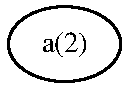
\includegraphics[scale=0.5]{image/example1}
\item \textit {t(s) = a(2)}
\item U({$H_s$}, 1) = \{a(2)\}
\item $\gamma_{t(s)}(V_{s})=\{a\}$ 
\end{itemize}

\item \textit {s = 3}
\begin{itemize}
\item We have: \textit {b(3)}
\item {$V_s$}= \{3\}
\item {$H_s$}= 
\includegraphics[scale=0.5]{image/example2}
\item \textit {t(s) = b(3)}
\item U({$H_s$}, 1) = \{b(3)\}
\item $\gamma_{t(s)}(V_{s})=\{b\}$ 
\end{itemize}

\item $s=2\oplus3$
\begin{itemize}
\item We have: $a(2)\oplus b(3)$
\item Apply (a) $\Longrightarrow\eta_{a,b}(a(2)\oplus b(3))$
\item {$V_s$}= \{2, 3\} 
\item {$H_s$}= 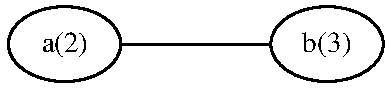
\includegraphics[scale=0.5]{image/example3}
\item U({$H_s$}, 1) = \{a(2)\}, U({$H_s$}, 2) =
\{b(3)\} 
\item $t(s)=\eta_{a,b}(a(2)\oplus b(3))$ 
\item $\gamma_{t(s)}(V_{s})=\{a,b\}$ 
\end{itemize}

\item $s=1\oplus(2\oplus3)$
\begin{itemize}
\item We have: $c(1)\oplus\eta_{a,b}(a(2)\oplus b(3))$
\item Apply (2) $\Longrightarrow\eta_{c,a}(c(1)\oplus\eta_{a,b}(a(2)\oplus b(3)))$
\item {$V_s$}= \{1, 2, 3\} 
\item {$H_s$} = 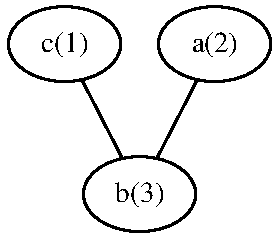
\includegraphics[scale=0.5]{image/example4}
\item U({$H_s$}, 1) = \{c(1), a(2)\}, U({$H_s$},
2) = \{b(3)\} 
\item Apply (c) $\Longrightarrow t(s)=\rho_{c\rightarrow a}(\eta_{c,a}(c(1)\oplus\eta_{a,b}(a(2)\oplus b(3))))$ 
\item $\gamma_{t(s)}(V_{s})=\{a,b\}$ 
\end{itemize}

\item $s=(1\oplus(2\oplus3))\oplus4$
\begin{itemize}
\item We have: $\rho_{c\rightarrow a}(\eta_{c,a}(c(1)\oplus\eta_{a,b}(a(2)\oplus b(3))))\oplus c(4)$
\item Apply (2) $\Longrightarrow\eta_{c,b}(\rho_{c\rightarrow a}(\eta_{c,a}(c(1)\oplus\eta_{a,b}(a(2)\oplus b(3))))\oplus c(4))$
\item {$V_s$}= \{1, 2, 3, 4\} 
\item {$H_s$} = 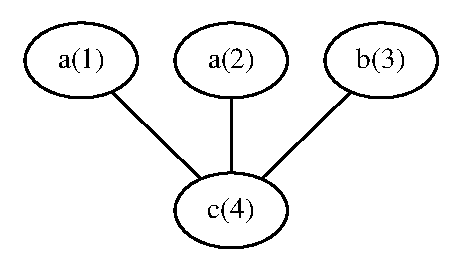
\includegraphics[scale=0.5]{image/example5}
\item U({$H_s$}, 1) = \{a(1), a(2), b(3)\}, U({$H_s$},
2) = \{c(4)\} 
\item Apply (c) $\Longrightarrow t(s)=\rho_{b\rightarrow a}(\eta_{c,b}(\rho_{c\rightarrow a}(\eta_{c,a}(c(1)\oplus\eta_{a,b}(a(2)\oplus b(3))))\oplus c(4)))$ 
\item $\gamma_{t(s)}(V_{s})=\{a,c\}$ 
\end{itemize}

\item $s=((1\oplus(2\oplus3))\oplus4)\oplus5$
\begin{itemize}
\item We have: $\rho_{b\rightarrow a}(\eta_{c,b}(\rho_{c\rightarrow a}(\eta_{c,a}(c(1)\oplus\eta_{a,b}(a(2)\oplus b(3))))\oplus c(4)))\oplus b(5)$
\item Apply (a) $\Longrightarrow\eta_{b,c}(\rho_{b\rightarrow a}(\eta_{c,b}(\rho_{c\rightarrow a}(\eta_{c,a}(c(1)\oplus\eta_{a,b}(a(2)\oplus b(3))))\oplus c(4)))\oplus b(5))$
\item {$V_s$}= \{1, 2, 3, 4, 5\} 
\item {$H_s$} = 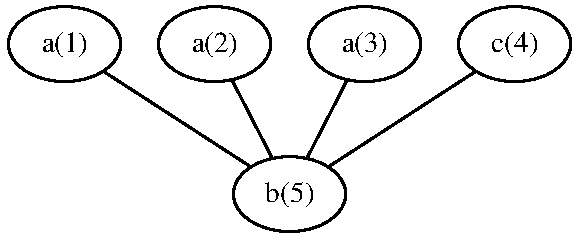
\includegraphics[scale=0.5]{image/example6}
\item U({$H_s$}, 1) = \{a(1), a(2), a(3), c(4)\}, U({$H_s$},
2) = \{b(5)\} 
\item Apply (c) $\Longrightarrow t(s)=\rho_{c\rightarrow a}(\eta_{b,c}(\rho_{b\rightarrow a}(\eta_{c,b}(\rho_{c\rightarrow a}(\eta_{c,a}(c(1)\oplus\eta_{a,b}(a(2)\oplus b(3))))\oplus c(4)))\oplus b(5)))$ 
\item $\gamma_{t(s)}(V_{s})=\{a,b\}$ 
\end{itemize}

\item $s=(((1\oplus(2\oplus3))\oplus4)\oplus5)\oplus6$
\begin{itemize}
\item We have: $\rho_{c\rightarrow a}(\eta_{b,c}(\rho_{b\rightarrow a}(\eta_{c,b}(\rho_{c\rightarrow a}(\eta_{c,a}(c(1)\oplus\eta_{a,b}(a(2)\oplus b(3))))\oplus c(4)))\oplus b(5)))\oplus c(6)$
\item Apply (a) $\Longrightarrow\eta_{c,b}(\rho_{c\rightarrow a}(\eta_{b,c}(\rho_{b\rightarrow a}(\eta_{c,b}(\rho_{c\rightarrow a}(\eta_{c,a}(c(1)\oplus\eta_{a,b}(a(2)\oplus b(3))))\oplus c(4)))\oplus b(5)))\oplus c(6))$
\item {$V_s$}= \{1, 2, 3, 4, 5, 6\} 
\item {$H_s$} = 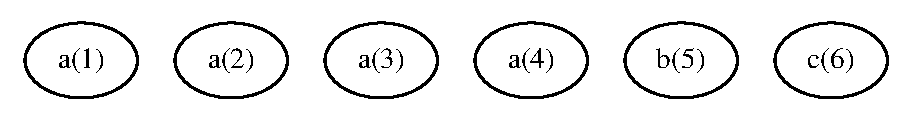
\includegraphics[scale=0.5]{image/example7}
\item U({$H_s$}, 1) = \{a(1), a(2), a(3), c(4), b(5), c(6)\} 
\item Apply (c) $\Longrightarrow t(s)=\rho_{c\rightarrow a}(\rho_{b\rightarrow a}(\eta_{c,b}(\rho_{c\rightarrow a}(\eta_{b,c}(\rho_{b\rightarrow a}(\eta_{c,b}(\rho_{c\rightarrow a}(\eta_{c,a}(c(1)\oplus\eta_{a,b}(a(2)\oplus b(3))))\oplus c(4)))\oplus b(5)))\oplus c(6))))$ 
\item $\gamma_{t(s)}(V_{s})=\{a\}$ 
\end{itemize}
\end{enumerate}

% Test case for second graph %
\section{Test case for first graph}

In this section, we introduce some more test cases for the first graph, which was presented in sub section 2.5 \\

\begin{figure}[H]
\centering{}
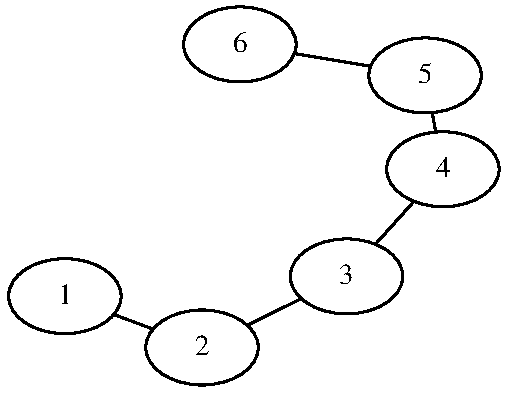
\includegraphics{image/graph_example}
\end{figure}

\begin{itemize}

\item Test case 1
	\begin{itemize}
		\item Edges: ((1,2),(2,3),(3,4),(4,5),(5,6))
		\item Sequence of vertices: 1, 2, 3, 4, 5, 6
		\item Linear reduced term: oplus(oplus(oplus(oplus(1,oplus(2,3)),4),5),6)
		\item Term: \seqsplit{rel\_c\_a[rel\_b\_a[add\_c\_b[oplus(rel\_c\_a[add\_b\_c[oplus(rel\_b\_a[add\_c\_a[oplus(rel\_c\_b[add\_c\_b[oplus(add\_b\_a[oplus(a(3),b(2))],c(1))]],c(4))]],b(5))]],c(6))]]]}
		\item Number of labels: 3
	\end{itemize}

\item Test case 2
	\begin{itemize}
		\item Edges: ((6,5),(5,4),(4,3),(3,2),(2,1))
		\item Sequence of vertices: 
		\item Linear reduced term: oplus(1, oplus(4, oplus(6, oplus(2, oplus(5, 3)))))
		\item Term: \seqsplit{rel\_c\_a[rel\_b\_a[add\_b\_c[oplus(rel\_d\_a[rel\_b\_a[add\_b\_a[oplus(rel\_b\_a[add\_d\_b[oplus(add\_c\_a[oplus(oplus(a(3),b(5)),c(2))],d(6))]],b(4))]]],b(1))]]]}
		\item Number of labels: 4
	\end{itemize}

\item Test case 3
	\begin{itemize}
		\item Edges: ((1,2),(2,3),(3,4),(4,5),(5,6))
		\item Sequence of vertices: 1, 4, 2, 5, 3, 6
		\item Linear reduced term: oplus(1, oplus(4, oplus(2, oplus(5, oplus(3, 6)))))
		\item Term: \seqsplit{rel\_d\_a[rel\_b\_a[add\_b\_d[oplus(rel\_c\_a[rel\_b\_a[add\_c\_b[oplus(rel\_c\_b[add\_d\_b[oplus(add\_c\_a[oplus(oplus(a(6),b(3)),c(5))],d(2))]],c(4))]]],b(1))]]]}
		\item Number of labels: 4
	\end{itemize}

\item Test case 4
	\begin{itemize}
		\item Edges: ((1,2),(2,3),(3,4),(4,5),(5,6))
		\item Sequence of vertices: 1, 3, 5, 6, 4, 2
		\item Linear reduced term: oplus(1, oplus(3, oplus(5, oplus(6, oplus(4, 2)))))
		\item Term: \seqsplit{rel\_c\_a[rel\_b\_a[add\_c\_a[oplus(rel\_d\_b[rel\_c\_b[add\_d\_b[add\_d\_a[oplus(rel\_d\_c[add\_d\_c[add\_d\_b[oplus(oplus(oplus(a(2),b(4)),c(6)),d(5))]]],d(3))]]]],c(1))]]]}
		\item Number of labels: 4
	\end{itemize}

\item Test case 5
	\begin{itemize}
		\item Edges: ((4,3),(4,5),(6,5),(1,2),(2,3))
		\item Sequence of vertices: 1, 3, 6, 5, 4, 2
		\item Linear reduced term: oplus(1, oplus(3, oplus(6, oplus(5, oplus(4, 2)))))
		\item Term: \seqsplit{rel\_c\_a[rel\_b\_a[add\_c\_a[oplus(rel\_d\_b[rel\_c\_b[add\_d\_b[add\_d\_a[oplus(rel\_d\_c[add\_d\_c[oplus(add\_c\_b[oplus(oplus(a(2),b(4)),c(5))],d(6))]],d(3))]]]],c(1))]]]}
		\item Number of labels: 4
	\end{itemize}

\item Test case 6
	\begin{itemize}
		\item Edges: ((5,4),(6,5),(2,1),(3,2),(4,3))
		\item Sequence of vertices: 6, 5, 1, 3, 4, 2
		\item Linear reduced term: oplus(6, oplus(5, oplus(1, oplus(oplus(3,4),2))))
		\item Term: \seqsplit{rel\_c\_a[rel\_b\_a[add\_b\_c[oplus(rel\_b\_a[add\_c\_a[oplus(rel\_d\_b[rel\_c\_b[add\_d\_c[oplus(add\_c\_b[oplus(add\_b\_a[oplus(a(4),b(3))],c(2))],d(1))]]],c(5))]],b(6))]]]}
		\item Number of labels: 4
	\end{itemize}

\item Test case 7
	\begin{itemize}
		\item Edges: ((1,2),(6,5),(4,5),(3,4),(2,3))
		\item Sequence of vertices: 1, 3, 5, 2, 6, 4
		\item Linear reduced term: oplus(oplus(oplus(1,oplus(oplus(3,5),2)),6),4)
		\item Term: \seqsplit{rel\_c\_a[rel\_b\_a[add\_b\_a[oplus(rel\_d\_c[rel\_b\_a[add\_d\_a[oplus(rel\_d\_c[add\_d\_c[oplus(add\_c\_b[oplus(oplus(a(5),b(3)),c(2))],d(1))]],d(6))]]],b(4))]]]}
		\item Number of labels: 4
	\end{itemize}
\end{itemize}

% Test case for second graph %
\section{Test case for second graph}
The second graph is

\begin{figure}[H]
\centering{}
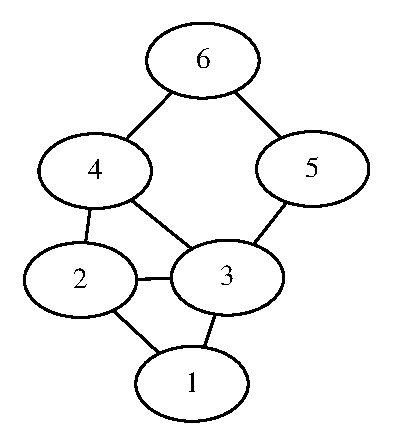
\includegraphics{image/graph2_example2}
\end{figure}

\begin{itemize}

\item Test case 1
	\begin{itemize}
		\item Edges: ((1,2),(1,3),(2,3),(2,4),(3,4),(3,5),(4,6),(5,6))
		\item Sequence of vertices: 1, 2, 3, 4, 5, 6
		\item Linear reduced term: oplus(1, oplus(2, oplus(3, oplus(4, oplus(5, 6)))))
		\item Term: \seqsplit{rel\_c\_a[rel\_b\_a[add\_c\_b[oplus(rel\_d\_b[rel\_c\_a[add\_b\_d[add\_b\_c[oplus(rel\_b\_a[add\_d\_c[add\_d\_b[oplus(add\_c\_a[oplus(add\_b\_a[oplus(a(6),b(5))],c(4))],d(3))]]],b(2))]]]],c(1))]]]}
		\item Number of labels: 4
	\end{itemize}

\item Test case 2
	\begin{itemize}
		\item Edges: ((2,3),(2,4),(3,1),(1,2),(4,3),(6,4),(6,5),(3,5))
		\item Sequence of vertices: 2, 6, 3 5, 4, 1
		\item Linear reduced term: oplus(2,oplus(6,oplus(oplus(oplus(3,5),4),1)))
		\item Term: \seqsplit{rel\_c\_a[rel\_b\_a[add\_c\_b[oplus(rel\_d\_a[rel\_c\_b[add\_d\_c[add\_d\_a[oplus(rel\_d\_b[add\_d\_b[oplus(add\_c\_b[oplus(add\_b\_a[oplus(a(5),b(3))],c(4))],d(1))]],d(6))]]]],c(2))]]]}
		\item Number of labels: 4
	\end{itemize}

\item Test case 3
	\begin{itemize}
		\item Edges: ((3,4),(4,6),(6,5),(5,3),(4,2),(2,1),(2,3),(1,3))
		\item Sequence of vertices: 1, 3, 5, 6, 4, 2
		\item Linear reduced term: oplus(oplus(oplus(oplus(1,oplus(3,5)),6),4),2)
		\item Term: \seqsplit{rel\_c\_a[rel\_b\_a[add\_c\_b[oplus(rel\_e\_b[rel\_d\_a[rel\_c\_b[add\_e\_d[add\_e\_b[oplus(add\_d\_a[oplus(add\_c\_b[oplus(add\_b\_a[oplus(a(5),b(3))],c(1))],d(6))],e(4))]]]]],c(2))]]]}
		\item Number of labels: 5
	\end{itemize}

\item Test case 4
	\begin{itemize}
		\item Edges: ((1,3),(3,5),(5,6),(6,4),(4,2),(2,1),(3,2),(3,4))
		\item Sequence of vertices: 4, 6, 3, 5, 1, 2
		\item Linear reduced term: oplus(4,oplus(6,oplus(oplus(oplus(3,5),1),2)))
		\item Term: \seqsplit{rel\_c\_a[rel\_b\_a[add\_c\_b[oplus(rel\_d\_b[rel\_c\_a[add\_d\_a[oplus(rel\_d\_b[add\_d\_c[add\_d\_b[oplus(add\_c\_b[oplus(add\_b\_a[oplus(a(5),b(3))],c(1))],d(2))]]],d(6))]]],c(4))]]]}
		\item Number of labels: 4
	\end{itemize}

\item Test case 5
	\begin{itemize}
		\item Edges: ((2,4),(4,6),(1,3),(3,5),(5,6),(2,1),(3,2),(3,4))
		\item Sequence of vertices: 2, 4, 6, 5, 3, 1
		\item Linear reduced term: oplus(2,oplus(4,oplus(oplus(oplus(6,5),3),1)))
		\item Term: \seqsplit{rel\_c\_a[rel\_b\_a[add\_b\_c[oplus(rel\_e\_c[rel\_d\_c[rel\_b\_a[add\_e\_c[add\_e\_b[oplus(add\_d\_c[oplus(add\_c\_a[oplus(add\_b\_a[oplus(a(5),b(6))],c(3))],d(1))],e(4))]]]]],b(2))]]]}
		\item Number of labels: 5
	\end{itemize}

\item Test case 6
	\begin{itemize}
		\item Edges: ((3,1),(3,2),(3,4),(3,5),(1,2),(5,6),(4,2),(4,6))
		\item Sequence of vertices: 3, 5, 2, 1, 4, 6
		\item Linear reduced term: oplus(3,oplus(5,oplus(2,oplus(oplus(1,4),6))))
		\item Term: \seqsplit{rel\_c\_a[rel\_b\_a[add\_b\_a[oplus(rel\_b\_a[add\_b\_c[oplus(rel\_b\_a[add\_b\_a[oplus(rel\_b\_a[add\_c\_a[oplus(oplus(a(4),b(1)),c(6))]],b(2))]],b(5))]],b(3))]]]}
		\item Number of labels: 3
	\end{itemize}

\item Test case 7
	\begin{itemize}
		\item Edges: ((6,5),(5,3),(3,1),(1,2),(2,4),(4,6),(4,3),(3,2))
		\item Sequence of vertices: 6, 5, 4, 1, 2, 3
		\item Linear reduced term: oplus(6,oplus(5,oplus(4,oplus(1,oplus(2,3)))))
		\item Term: \seqsplit{rel\_c\_a[rel\_b\_a[add\_b\_c[oplus(rel\_d\_c[rel\_b\_a[add\_c\_a[oplus(rel\_c\_b[add\_d\_b[add\_d\_a[oplus(add\_c\_b[add\_c\_a[oplus(add\_b\_a[oplus(a(3),b(2))],c(1))]],d(4))]]],c(5))]]],b(6))]]]}
		\item Number of labels: 4
	\end{itemize}
\end{itemize}


\end{document}